\documentclass[11pt,a4paper]{article}

% ---------------------------------------------------------------------------
% Elementary cores, abundant reactions, and the union-closed boundary of
% autocatalytic reaction systems.
%
% Author metadata: set the three macros below before submission.
% ---------------------------------------------------------------------------
\newcommand{\PaperAuthor}{Author name to be inserted}
\newcommand{\PaperAffiliation}{Affiliation to be inserted}
\newcommand{\PaperDate}{13 September 2026}

\usepackage[T1]{fontenc}
\usepackage[utf8]{inputenc}
\usepackage{lmodern}
\usepackage{microtype}
\usepackage[a4paper,margin=1.05in]{geometry}
\usepackage{amsmath,amssymb,amsthm,mathtools}
\usepackage{booktabs}
\usepackage{array}
\usepackage{enumitem}
\usepackage{xcolor}
\usepackage{tikz}
\usetikzlibrary{arrows.meta,positioning,fit,calc}
\usepackage[numbers,sort&compress]{natbib}
\usepackage[colorlinks=true,linkcolor=blue!55!black,citecolor=blue!55!black,urlcolor=blue!55!black]{hyperref}
\hypersetup{pdftitle={Elementary cores, abundant reactions, and the union-closed boundary of autocatalytic reaction systems},
  pdfkeywords={autocatalytic sets, RAF, union-closed sets conjecture, interior operators, antimatroids, Horn functions, Lean}}

\DeclareUrlCommand\lean{\urlstyle{tt}}
\setlist{itemsep=2pt,topsep=3pt}
\setlength{\emergencystretch}{1.5em}

\theoremstyle{plain}
\newtheorem{theorem}{Theorem}[section]
\newtheorem{proposition}[theorem]{Proposition}
\newtheorem{lemma}[theorem]{Lemma}
\newtheorem{corollary}[theorem]{Corollary}
\theoremstyle{definition}
\newtheorem{definition}[theorem]{Definition}
\newtheorem{example}[theorem]{Example}
\newtheorem{construction}[theorem]{Construction}
\newtheorem{question}[theorem]{Question}
\theoremstyle{remark}
\newtheorem{remark}[theorem]{Remark}

\newcommand{\FF}{\mathcal F}
\newcommand{\AAf}{\mathcal A}
\newcommand{\DD}{\mathcal D}
\newcommand{\BB}{\mathcal B}
\newcommand{\GG}{\mathcal G}
\newcommand{\HH}{\mathcal H}
\newcommand{\QQ}{\mathcal Q}
\newcommand{\cl}{\operatorname{cl}}
\newcommand{\enc}{\operatorname{enc}}
\newcommand{\mraf}{\operatorname{maxRAF}}
\newcommand{\R}{\mathbb R}
\newcommand{\N}{\mathbb N}
\DeclareMathOperator{\Fix}{Fix}

\title{Elementary cores, abundant reactions, and the union-closed\\ boundary of autocatalytic reaction systems}
\author{\PaperAuthor\\[2pt] {\small\itshape \PaperAffiliation}}
\date{\PaperDate}

\begin{document}
\maketitle

\begin{abstract}
A reflexively autocatalytic and food-generated set (RAF) of a catalytic reaction
system is a collection of reactions that can be built up from a food set and in
which every reaction is catalysed from within. The RAFs of a finite system, with
the empty set adjoined, form a union-closed family, and Steel asked whether some
reaction always lies in at least half of its members: a RAF form of Frankl's
union-closed sets conjecture. We prove this for every system that contains a
\emph{viable elementary core}, a nonempty RAF all of whose reactants are food,
with no restriction on the remaining reactions or on catalytic feedback into
the core. The proof conditions on the reactions selected outside the core,
recomputes the core's support relation in that context, and applies the
Horn-function counting injection of Lozin and Zamaraev to the resulting support
relation under an upward constraint. The occupancy inequality holds separately in every
exterior context, survives arbitrary nonnegative weights on contexts, and
implies that every catalytic cycle of food-ready reactions meets a globally
abundant reaction, that vertex-disjoint cycles yield distinct abundant
reactions, and that systems with at most two non-food-ready reactions satisfy
the half-frequency bound. Sharpness and a changing-witness example are given,
together with exact projection diagnostics for an embedded module.
We then locate the boundary of the method. RAF interior operators on a fixed
reaction set are characterised as accessible union-closed food feasibility
intersected with predecessor support; food-generation families are exactly
antimatroids. A producer--gate construction with two reactions per coordinate
realises every finite union-closed family containing the empty set, preserving
frequencies and all availability queries with one food molecule, one catalyst per
reaction, and molecular closure stabilising after two rounds. Its elementary RAFs
correspond exactly to the singleton members of the encoded family. Hence a
half-frequency theorem for systems without an elementary core is equivalent to the
unrestricted union-closed conjecture, which remains open. The main theorems are
verified in Lean~4 against Mathlib; the correspondence between the article and
the formal development is recorded in an appendix.
\end{abstract}

\noindent\textbf{Keywords.} autocatalytic sets; RAF theory; union-closed sets conjecture; interior operators; antimatroids; Horn functions; formal verification.

\noindent\textbf{MSC 2020.} 05D05, 92C42, 06A15, 68V20.

\section{Introduction}\label{sec:intro}

\subsection{Autocatalytic sets and the RAF formalism}

Collectively autocatalytic sets were proposed by Kauffman~\cite{kauffman1986autocatalytic,kauffman1993origins}
as a route by which a mixture of simple molecules could organise into a self-sustaining
chemistry: a set of reactions each of whose products is needed, as reactant or
catalyst, by other reactions of the set, so that the set as a whole reproduces
itself from an ambient food supply. Hordijk and Steel~\cite{hordijk2004detecting}
made this precise in the RAF formalism. A \emph{catalytic reaction system}
consists of molecule types, reactions with reactant and product sets, a
distinguished \emph{food} set, and a catalysis relation. A set of reactions is
\emph{food-generated} if its reactants can all be produced, in some order, from
food using only the selected reactions, and it is \emph{reflexively autocatalytic}
if every selected reaction has a catalyst that is food or produced by the
selected reactions. A RAF is a nonempty set that is both. Hordijk and Steel gave a
polynomial-time algorithm for the largest RAF inside any given set of reactions,
and the formalism has since been developed extensively; we refer to
\cite{hordijk2017chasing,steel2019autocatalytic,mossel2005random} for structural
theory, algorithms, and random-network analysis.

The union of two RAFs is again a RAF. Adjoining the empty set, the RAFs of a
finite system therefore form a \emph{union-closed family} of subsets of the
reaction set, and the map sending an available reaction set to the largest RAF it
contains is an \emph{interior operator}: contractive, monotone and idempotent.
Steel~\cite{steel2023interior} studied this operator in detail and, in his
concluding section, asked
\begin{quote}
``whether there is always a reaction that lies in at least half the RAFs (for either an elementary or general CRS).''
\end{quote}
Here \emph{elementary} means that every reaction has all its reactants in the food set.
Since the RAF family is union-closed, a positive answer for all systems would follow
from Frankl's union-closed sets conjecture~\cite{frankl1995extremal,bruhn2015journey}, which asserts
that every finite union-closed family other than $\{\varnothing\}$ has an element
lying in at least half of its members. That conjecture is open. After a long period
in which only logarithmic bounds were known~\cite{wojcik1999union}, Gilmer~\cite{gilmer2022constant}
proved a constant lower bound of $0.01$ by an entropy argument, quickly improved to
$(3-\sqrt5)/2\approx0.382$ and beyond~\cite{alweiss2022improved,chase2022approximate,sawin2022improved,cambie2022better};
the constant $1/2$ remains out of reach.

The question for RAF systems has two faces. Does the chemical structure of a RAF family
make the half-frequency statement provable where it is not provable for arbitrary union-closed
families? Or is every union-closed family already a RAF family in disguise, so that the RAF
question is exactly as hard as Frankl's? This paper answers both questions as precisely as
we are able: the first positively for a large structurally defined class, the second positively
for the complement of that class.

\subsection{Main results}

Throughout, $\FF(\QQ)$ denotes the family of RAFs of a finite catalytic reaction system $\QQ$
together with the empty set, $N=|\FF(\QQ)|$, and $f(r)$ is the number of members containing
the reaction $r$. A reaction is \emph{abundant} if $2f(r)\ge N$. Because the empty set
contributes to the denominator but to no numerator, abundance is slightly stronger than the
half-frequency statement over nonempty RAFs alone; Steel's question is the weaker form, and
all our positive results give the stronger one.

A reaction is \emph{food-ready} if all its reactants are food. An \emph{elementary core} of
$\QQ$ is a nonempty RAF of $\QQ$ consisting of food-ready reactions. The core is a subset
of a system that may otherwise be entirely unrestricted.

\begin{theorem}[Elementary-core abundance; Theorem~\ref{thm:core}]\label{thm:intro-core}
Let $U$ be an elementary core of a finite catalytic reaction system $\QQ$. Then some
reaction of $U$ is abundant in $\FF(\QQ)$. More precisely, for every set $T$ of reactions
outside $U$, the core parts $S=W\cap U$ of the members $W\in\FF(\QQ)$ with $W\setminus U=T$
have average size at least $|U|/2$.
\end{theorem}

The fibrewise form is the real content. Fixing the exterior selection $T$ changes which
core reactions are catalysed from outside; the proof recomputes the internal support
relation of $U$ in the presence of $T$ and shows that the family of compatible core subsets
is always a ``supported family under an upward constraint'', for which a counting injection
gives average size at least half the ground set. The counting injection is the
horizontal/vertical cell map of Lozin and Zamaraev~\cite{lozin2024union}, who used it to
prove Frankl's conjecture for Horn functions with a \emph{dependency property}; an upward
constraint is a positive Boolean predicate and satisfies that property vacuously, so the
lemma we need (Lemma~\ref{lem:count}) is the aggregate form of their theorem. No assumption is
made that the exterior preserves the isolated support structure of the core; indeed we exhibit
systems where it does not (Section~\ref{sec:diagnostics}).

The fibrewise inequality has several consequences that a bare existence statement would not
give (Section~\ref{sec:consequences}). The half bound survives any nonnegative reweighting of
exterior contexts; every directed cycle in the food-ready support digraph contains a globally
abundant reaction, so the strictly rare food-ready reactions induce an acyclic subgraph and
$k$ vertex-disjoint cycles force $k$ distinct abundant reactions; and any system with a RAF
and at most two non-food-ready reactions has an abundant reaction, by a separate two-element
transversal argument. The constant $1/2$ is attained, and the abundant reaction inside the
core may depend on the exterior context (Example~\ref{ex:switch}).

The second group of results describes what RAF families can be (Sections~\ref{sec:realization}--\ref{sec:pair}).

\begin{theorem}[Exact-ground realizability; Theorem~\ref{thm:same}]\label{thm:intro-same}
An interior operator on $2^V$ is the RAF interior operator of a finite catalytic reaction
system with reaction set exactly $V$ if and only if its fixed family is the intersection of
an accessible union-closed family containing $\varnothing$ with a predecessor-support family
$\{S:\ S\cap P(v)\neq\varnothing\text{ for all }v\in S\}$.
In particular the families of food-generated sets are exactly the finite antimatroids
(Corollary~\ref{cor:antimatroid}).
\end{theorem}

\begin{theorem}[Sparse universality; Theorem~\ref{thm:pair} and Proposition~\ref{prop:paircore}]\label{thm:intro-pair}
Every finite union-closed family $\DD\subseteq2^V$ containing $\varnothing$ is, up to the
bijection $A\mapsto\{p_v,g_v:v\in A\}$, the RAF family of a system with $2|V|$ reactions,
one food molecule, exactly one catalyst per reaction, no self-catalysis, catalytic
product edges forming disjoint two-cycles, and molecular closure stabilising after two
rounds for every availability set. The bijection preserves frequencies and translates
every maxRAF query into an interior query on complete pairs. The elementary RAFs of this
system are the encodings of the singleton members of $\DD$.
\end{theorem}

Since a union-closed family with a singleton member trivially has an abundant element,
Theorem~\ref{thm:intro-pair} shows that the class of systems \emph{without} an elementary
core carries the full difficulty of the union-closed conjecture: a half-frequency theorem
for that class is equivalent to Frankl's conjecture (Theorem~\ref{thm:equiv}). The pair of
theorems thus draws a sharp line. On one side, elementary cores force abundance with room
to spare; on the other, no amount of structural sparsity in the catalytic graph helps, because
the difficulty is carried entirely by reactant requirements.

\subsection{Relation to prior work and what is new}

The RAF framework, the maxRAF interior operator, and the question itself are due to
Hordijk and Steel~\cite{hordijk2004detecting} and Steel~\cite{steel2023interior}. The
characterisation of elementary RAFs by directed cycles in a support digraph, and the
shortest-cycle method for a smallest elementary RAF, appear in
Steel, Hordijk and Xavier~\cite{steel2019autocatalytic}; we use them as certificates
for abundance in a surrounding system. The counting kernel is Theorem~4 of Lozin and
Zamaraev~\cite{lozin2024union}, which proves Frankl's conjecture for Boolean functions
admitting a Horn DNF with their dependency property: every variable occurring negatively
has a companion variable occurring positively in each term in which it is negative. The
RAF family of an isolated elementary system is an instance. What is new here is (i) the
exterior-conditioned application, in which the Horn bodies depend on the fixed exterior
and food generation together with exterior support enter as a monotone constraint,
giving abundance for embedded cores under arbitrary feedback; (ii) the
weighting, cycle, disjointness and two-exception consequences; (iii) the exact-ground
characterisation and the antimatroid identification of food generation; and (iv) the
sparse producer--gate universality theorem with its exact elementary boundary and the
resulting equivalence with the unrestricted conjecture. We make no claim on the
unrestricted conjecture. A focused comparison with the sources cited is not a
certification of priority across the whole literature.

The classical observation that a union-closed family containing a singleton (or a
two-element set) satisfies the conjecture is due to Sarvate and Renaud~\cite{sarvate1989union}
(see also Poonen~\cite{poonen1992union}). Reimer's average set size
theorem~\cite{reimer2003average} gives average member size at least $\tfrac12\log_2 N$ for any
union-closed family; our occupancy inequalities are of the same average-size type but give
the much larger bound $|U|/2$ under the structural hypothesis, and only for the core
coordinates.

\subsection{Formal verification}

The theorems marked with a Lean identifier in Appendix~\ref{app:lean} have been formalised
in Lean~4~\cite{demoura2021lean} against Mathlib~\cite{mathlib2020} directly from the
literal RAF semantics of Definition~\ref{def:crs}, compiled with warnings as errors, and
depend only on the standard axioms \lean{Classical.choice}, \lean{Quot.sound} and
\lean{propext}. The paper is written to be read without the formal development; the
appendix states exactly which forms were compiled and which steps (a few reindexings and
the examples) are ordinary mathematics only.

\subsection{Organisation}

Section~\ref{sec:prelim} fixes the RAF semantics and basic facts. Section~\ref{sec:count}
proves the counting lemma. Section~\ref{sec:core} proves the exterior-conditioned abundance
theorem. Section~\ref{sec:consequences} derives the weighted, cycle, disjointness and
two-exception consequences and gives examples. Section~\ref{sec:diagnostics} gives exact
diagnostics for when an embedded module's isolated behaviour is visible globally.
Sections~\ref{sec:realization} and~\ref{sec:pair} contain the realisation theorems and the
equivalence with the unrestricted conjecture. Section~\ref{sec:algorithms} discusses
certificates and algorithms, and Section~\ref{sec:scope} states the limits of the results
and open problems. Appendix~\ref{app:lean} records the formal verification.

\section{Ordinary RAF semantics}\label{sec:prelim}

\begin{definition}\label{def:crs}
A finite \emph{catalytic reaction system} (CRS) is a tuple $\QQ=(X,R,F,\rho,\pi,C)$ where
$X$ is a finite set of molecule types, $R$ a finite set of reactions, $F\subseteq X$ the
\emph{food} set, $\rho(r),\pi(r)\subseteq X$ the reactants and products of $r\in R$, and
$C\subseteq X\times R$ the catalysis relation; write $C(r)=\{x:(x,r)\in C\}$.
For $W\subseteq R$ define the \emph{molecular closure} stages
\[
L_0(W)=F,\qquad
L_{j+1}(W)=L_j(W)\cup\bigcup\{\pi(r):\ r\in W,\ \rho(r)\subseteq L_j(W)\},
\]
and the \emph{closure} $\cl_W(F)=\bigcup_{j\ge0}L_j(W)$.
$W$ is \emph{food-generated} if $\rho(r)\subseteq\cl_W(F)$ for every $r\in W$.
$W$ is a \emph{RAF} if it is nonempty, food-generated, and $C(r)\cap\cl_W(F)\ne\varnothing$
for every $r\in W$.
\end{definition}

Catalysis plays no role in the closure recursion: a reaction contributes its products
as soon as its reactants are present, and catalytic support is checked afterwards in
the resulting closure. This is the semantics of~\cite{hordijk2004detecting,steel2023interior};
we impose no stoichiometry, inhibition or kinetics. Since $X$ is finite the closure
stabilises after finitely many stages.

\begin{lemma}[Products identity]\label{lem:products}
Closure is monotone: $W\subseteq W'$ implies $L_j(W)\subseteq L_j(W')$ for all $j$.
If $W$ is food-generated then
\begin{equation}\label{eq:products}
\cl_W(F)=F\cup\pi(W),\qquad \pi(W):=\bigcup_{r\in W}\pi(r).
\end{equation}
\end{lemma}
\begin{proof}
Monotonicity is immediate by induction on $j$. Every stage adds only products of
reactions in $W$, so $\cl_W(F)\subseteq F\cup\pi(W)$. Conversely if $W$ is food-generated
and $r\in W$, then $\rho(r)\subseteq L_j(W)$ for some finite $j$, whence
$\pi(r)\subseteq L_{j+1}(W)$.
\end{proof}

Thus, \emph{for a food-generated set}, catalytic support is exactly support by food or by a
product of a selected reaction. The qualification matters: products of a selected reaction
that never becomes enabled are not available.

\begin{definition}\label{def:family}
For a finite CRS $\QQ$ put
\[
\FF=\FF(\QQ)=\{\varnothing\}\cup\{W\subseteq R:\ W\text{ is a RAF}\},\qquad N=|\FF|,\qquad
f(r)=|\{W\in\FF: r\in W\}|.
\]
A reaction is \emph{abundant} if $2f(r)\ge N$ and \emph{strictly rare} otherwise.
A reaction is \emph{food-ready} if $\rho(r)\subseteq F$. An \emph{elementary core} is a
nonempty RAF all of whose reactions are food-ready. For $A\subseteq R$,
$\mraf_\QQ(A)=\bigcup\{W\in\FF:W\subseteq A\}$.
\end{definition}

\begin{lemma}\label{lem:uc}
$\FF$ is union-closed. $\mraf_\QQ(A)$ is the largest RAF contained in $A$, or empty if there
is none, and $A\mapsto\mraf_\QQ(A)$ is an interior operator on $2^R$ with fixed family $\FF$.
\end{lemma}
\begin{proof}
If $W,W'$ are RAFs then $W\cup W'$ is nonempty; by monotonicity of closure each reaction of
$W\cup W'$ keeps its food generation and its catalyst. The union of all RAFs inside $A$ is
therefore a RAF or empty, and the remaining properties are immediate.
\end{proof}

Conversely, every interior operator $\psi$ on a finite power set is determined by its fixed
family $\Fix(\psi)$, which contains $\varnothing$ and is union-closed, via
$\psi(A)=\bigcup\{S\in\Fix(\psi):S\subseteq A\}$. We use ``interior operator'' and
``union-closed family containing $\varnothing$'' interchangeably. For such a family
$\DD\subseteq2^V$ we write $i_\DD(A)=\bigcup\{D\in\DD:D\subseteq A\}$.

\begin{remark}[Two normalisations of the conjecture]\label{rem:normal}
Steel's question concerns nonempty RAFs: is there $r$ with $f(r)\ge (N-1)/2$? Our
abundance condition $2f(r)\ge N$ is stronger. For the union-closed conjecture the two
normalisations are equivalent: applying the standard conjecture to $\DD\cup\{\varnothing\}$
gives the empty-inclusive bound, and the empty-inclusive bound for $\DD\cup\{\varnothing\}$
implies the standard bound for $\DD$ because the denominator can only grow. We work
exclusively with the empty-inclusive form because it is the one that sums correctly over
exterior fibres (the empty fibre member is a genuine row of the count).
\end{remark}

\section{Supported families under an upward constraint}\label{sec:count}

A predicate $K$ on $2^U$ is \emph{upward} if $K(S)$ and $S\subseteq S'$ imply $K(S')$.

\begin{lemma}[Occupancy of supported families]\label{lem:count}
Let $U$ be a finite set with $n=|U|$. For each $r\in U$ let $B_r\subseteq U$ be a nonempty
\emph{body}, and let $K$ be an upward predicate on $2^U$. Put
\[
\BB=\{S\subseteq U:\ K(S)\ \text{and}\ S\cap B_r\ne\varnothing\ \text{for every } r\in S\}.
\]
Then
\begin{equation}\label{eq:count}
\sum_{S\in\BB}\bigl(2|S|-n\bigr)\ \ge\ 0,
\qquad\text{equivalently}\qquad n\,|\BB|\le 2\sum_{S\in\BB}|S|.
\end{equation}
\end{lemma}

In words: if membership requires each selected element to be ``supported'' by a selected
element of its body, and is additionally restricted by any upward condition, then the
members have average size at least $n/2$. In Boolean terms, the complements of the members
are the false points of the DNF $P\vee\bigvee_r(\bar r\wedge\bigwedge_{p\in B_r}p)$, where
$P$ is the positive DNF of the failure of $K$. This DNF is Horn and has the dependency
property of Lozin and Zamaraev~\cite[Theorem~4]{lozin2024union}: the only term in which
$r$ occurs negatively contains any chosen $d(r)\in B_r$ positively, and the terms of $P$
contain no negative literal. Their proof shows that the matrix of true points has at least
as many ones as zeros, which is exactly~\eqref{eq:count} after complementation; they then
deduce a good variable, whereas we need the aggregate inequality itself. We include the
argument for completeness and because the formal development treats the upward predicate
abstractly rather than as a DNF.

\begin{proof}
Work in deletion coordinates $D=U\setminus S$, and call a row $D\subseteq U$ \emph{bad} if
$U\setminus D\notin\BB$. Set $P(D):\Leftrightarrow\neg K(U\setminus D)$ and, for $r\in U$,
\[
H_r(D):\Leftrightarrow\ r\notin D\ \text{and}\ B_r\subseteq D .
\]
Then $D$ is bad iff $P(D)$ or $H_r(D)$ for some $r$: indeed $S=U\setminus D$ fails
$S\cap B_r\neq\varnothing$ for some $r\in S$ exactly when $r\notin D$ and $B_r\subseteq D$.
Since $K$ is upward, $P$ is upward in $D$.

A \emph{cell} is a pair $(D,r)\in2^U\times U$; it is a \emph{zero cell} if $r\notin D$ and a
\emph{one cell} if $r\in D$. Fix a choice $d(r)\in B_r$ for each $r$. Define a map $\varphi$
on the zero cells of bad rows:
\begin{itemize}
\item[(H)] if $P(D)$ holds, or $H_q(D)$ holds for some $q\neq r$, let $\varphi(D,r)=(D\cup\{r\},\,r)$;
\item[(V)] otherwise let $\varphi(D,r)=(D,\,d(r))$.
\end{itemize}
Call the first kind of move horizontal and the second vertical.

\emph{Targets are one cells of bad rows.} In case (H), $r\in D\cup\{r\}$, and the row
$D\cup\{r\}$ is bad because $P$ persists upward, or because $q\notin D$ and $q\neq r$ give
$q\notin D\cup\{r\}$ while $B_q\subseteq D\subseteq D\cup\{r\}$. In case (V), $D$ is bad but
$P(D)$ fails, so some $H_q(D)$ holds, and by the case hypothesis $q=r$; hence
$B_r\subseteq D$ and $d(r)\in D$, so $(D,d(r))$ is a one cell of the bad row $D$.

\emph{$\varphi$ is injective.} Two horizontal sources with a common target
$(D\cup\{r\},r)$ have the same second coordinate $r$ and the same row after removing $r$,
so they coincide. Two vertical sources $(D,r),(D,r')$ with a common target lie in the same
row; verticality means that every covering term of $D$ has head $r$, and also head $r'$,
and since some covering term exists, $r=r'$. For a mixed collision let $(A,a)$ be
horizontal and $(D,b)$ vertical with $(A\cup\{a\},a)=(D,d(b))$; so $D=A\cup\{a\}$,
$a=d(b)$ and $a\notin A$. If $P(A)$ held then $P(D)$ would hold by upwardness, contradicting
verticality of $(D,b)$. Hence the horizontal move was justified by some $H_q(A)$ with
$q\neq a$. If $q=b$ then $B_b\subseteq A$, so $a=d(b)\in A$, a contradiction. If $q\neq b$
then $q\notin A$ and $q\neq a$ give $q\notin D$, and $B_q\subseteq A\subseteq D$, so
$H_q(D)$ holds with $q\neq b$, contradicting verticality. Thus $\varphi$ is injective.

\emph{Counting.} Let $Z_{\rm bad},O_{\rm bad}$ be the numbers of zero and one cells in bad
rows and $Z_{\rm good},O_{\rm good}$ those in good rows. The injection gives
$Z_{\rm bad}\le O_{\rm bad}$. The whole cube has $n2^{n-1}$ zero cells and $n2^{n-1}$ one
cells, so $Z_{\rm good}\ge O_{\rm good}$, that is
$\sum_{D\ \rm good}(n-|D|)\ge\sum_{D\ \rm good}|D|$. Writing $S=U\setminus D$, the good rows
are exactly the members of $\BB$ and $n-2|D|=2|S|-n$, which is~\eqref{eq:count}.
\end{proof}

\begin{remark}
The lemma is trivially true when $\BB=\varnothing$, and it is applied below with
$U$ nonempty. Only the finiteness of $U$, the nonemptiness of the bodies and the
upwardness of $K$ are used; the bodies may contain their own head (a self-supported
element), and $K$ may be false everywhere or true everywhere.
\end{remark}

\section{The exterior-conditioned abundance theorem}\label{sec:core}

\begin{theorem}[Elementary-core abundance, fibre form]\label{thm:core}
Let $U$ be an elementary core of a finite CRS $\QQ$, $n=|U|$. For $T\subseteq R\setminus U$
define the \emph{exterior fibre}
\[
\BB_T=\{S\subseteq U:\ S\cup T\in\FF(\QQ)\}.
\]
Then for every $T\subseteq R\setminus U$,
\begin{equation}\label{eq:fibre}
\sum_{S\in\BB_T}\bigl(2|S|-n\bigr)\ \ge\ 0 .
\end{equation}
Consequently
\begin{equation}\label{eq:global}
2\sum_{W\in\FF}|W\cap U|\ \ge\ nN,\qquad\text{and some } r\in U \text{ satisfies } 2f(r)\ge N .
\end{equation}
Nothing is assumed about the reactions outside $U$: they may have arbitrary reactants,
products and catalysts, including catalysts for reactions of $U$.
\end{theorem}

\begin{proof}
Fix $T\subseteq R\setminus U$. Call a core reaction $r\in U$ \emph{$T$-automatic} if
$C(r)\cap\bigl(F\cup\pi(T)\bigr)\neq\varnothing$, and define bodies
\[
B_r=\begin{cases}\{r\} & \text{if $r$ is $T$-automatic},\\[2pt]
\{p\in U:\ \pi(p)\cap C(r)\neq\varnothing\} & \text{otherwise.}\end{cases}
\]
Each $B_r$ is nonempty: if $r$ is not $T$-automatic then $C(r)\cap F=\varnothing$, while
$U$ is a RAF, so by Lemma~\ref{lem:products} $r$ has a catalyst in
$\cl_U(F)=F\cup\pi(U)$, hence in $\pi(p)$ for some $p\in U$. (Exterior support can only
enlarge the set of automatic heads; it never destroys an internal supplier.)

For $S\subseteq U$ let $K_T(S)$ assert that $S\cup T$ is food-generated and that every
$t\in T$ satisfies $C(t)\cap\bigl(F\cup\pi(S\cup T)\bigr)\neq\varnothing$. Then $K_T$ is
upward on $2^U$: if $S\subseteq S'$, every reaction of $S\cup T$ keeps its food generation
in $S'\cup T$ by monotonicity of closure, every reaction of $S'\setminus S$ is food-ready,
and $\pi(S\cup T)\subseteq\pi(S'\cup T)$.

We claim the exact identity
\begin{equation}\label{eq:exact-fibre}
\BB_T=\{S\subseteq U:\ K_T(S)\ \text{and}\ S\cap B_r\neq\varnothing\text{ for every }r\in S\}.
\end{equation}
If $S\cup T=\varnothing$ both sides contain $S=\varnothing$ (all conditions are vacuous), so
assume $S\cup T\neq\varnothing$. Suppose $S\cup T\in\FF$, i.e. it is a RAF. Then $S\cup T$
is food-generated, and by~\eqref{eq:products} every $t\in T$ has a catalyst in
$F\cup\pi(S\cup T)$, so $K_T(S)$ holds. Let $r\in S$. If $r$ is $T$-automatic then
$r\in S\cap B_r$. Otherwise $r$ has a catalyst in $F\cup\pi(S\cup T)$ but none in
$F\cup\pi(T)$, so some $p\in S$ has $\pi(p)\cap C(r)\neq\varnothing$, i.e. $p\in S\cap B_r$.
Conversely suppose $K_T(S)$ and $S\cap B_r\neq\varnothing$ for all $r\in S$. Then $S\cup T$
is nonempty and food-generated, so $\cl_{S\cup T}(F)=F\cup\pi(S\cup T)$; each $t\in T$ is
catalysed from this closure by $K_T$; a $T$-automatic $r\in S$ is catalysed from
$F\cup\pi(T)\subseteq\cl_{S\cup T}(F)$; and a non-automatic $r\in S$ has some $p\in S$ with
$\pi(p)\cap C(r)\neq\varnothing$ and $\pi(p)\subseteq\cl_{S\cup T}(F)$. So $S\cup T$ is a RAF.

Lemma~\ref{lem:count} applied to the bodies $B_r$ and the upward predicate $K_T$ now
gives~\eqref{eq:fibre}. Note that $T$ itself need not be food-generated or a RAF; its
products are usable as catalysts only jointly with the requirement that $S\cup T$ be
food-generated, which is part of $K_T$.

For~\eqref{eq:global}, every $W\in\FF$ is uniquely $W=S\cup T$ with $T=W\setminus U$ and
$S=W\cap U\in\BB_T$, and conversely $S\cup T\in\FF$ for every $T\subseteq R\setminus U$ and
$S\in\BB_T$. Summing~\eqref{eq:fibre} over $T$ gives
$\sum_{W\in\FF}(2|W\cap U|-n)\ge0$. Finally $\sum_{W\in\FF}|W\cap U|=\sum_{r\in U}f(r)$, so
$\sum_{r\in U}f(r)\ge nN/2$, and as $U\neq\varnothing$ some $r\in U$ has $f(r)\ge N/2$.
\end{proof}

\begin{remark}[What the theorem does not assert]
The abundant reaction is not identified by the proof, only located in $U$; different
exterior contexts may be balanced by different core reactions (Example~\ref{ex:switch}).
The proof does not interchange quantifiers: it derives a single global witness from the
aggregate incidence inequality, not from fibrewise witnesses. The hypothesis is a
\emph{viable} elementary core: a food-ready set that fails to be a RAF on its own does not
qualify, even if it becomes viable with exterior help.
\end{remark}

\begin{remark}[Fibre slack]\label{rem:slack}
Define the slack of a context by $\sigma(T)=\sum_{S\in\BB_T}(2|S|-n)\ge0$. The proof shows
the exact identity
\[
2\sum_{r\in U}f(r)-nN=\sum_{T\subseteq R\setminus U}\sigma(T),
\]
so the global surplus over the half bound decomposes exactly into the contexts in which the
occupancy inequality is strict. Example~\ref{ex:switch} has $\sigma\equiv0$.
\end{remark}

\begin{remark}[Comparison with an isolated argument]
For the isolated elementary system $\QQ|_U$ (exterior deleted) the fibre $\BB_\varnothing$
is its own RAF family, all $K_\varnothing(S)$ hold, and~\eqref{eq:fibre} is the
Lozin--Zamaraev theorem for the Horn function ``every selected head has a selected
supplier''. The point of Theorem~\ref{thm:core} is that an exterior with feedback changes
both the bodies (heads become automatic) and the admissible rows (through $K_T$), and the
counting lemma is indifferent to both changes.
\end{remark}

\section{Consequences}\label{sec:consequences}

\subsection{Weighting and conditioning}

\begin{corollary}[Exterior weighting]\label{cor:weight}
Under the hypotheses of Theorem~\ref{thm:core}, let $h:2^{R\setminus U}\to\R_{\ge0}$. Then
\begin{equation}\label{eq:weight}
\sum_{W\in\FF}h(W\setminus U)\,\bigl(2|W\cap U|-n\bigr)\ \ge\ 0 .
\end{equation}
If $Z=\sum_{W\in\FF}h(W\setminus U)>0$, some $r\in U$ satisfies
$\sum_{W\in\FF,\ r\in W}h(W\setminus U)\ \ge\ Z/2$.
\end{corollary}
\begin{proof}
Multiply~\eqref{eq:fibre} by $h(T)\ge0$ and sum over $T$; reindexing by $W=S\cup T$
gives~\eqref{eq:weight}. Then
$2\sum_{r\in U}\sum_{W\ni r}h(W\setminus U)=2\sum_W h(W\setminus U)|W\cap U|\ge nZ$, and
averaging over the $n$ elements of $U$ gives the witness.
\end{proof}

Indicator weights $h=\mathbf 1_{\mathcal T}$ condition on any collection $\mathcal T$ of
exterior contexts, including a single nonempty fibre. Choosing $h(T)=q(T)/|\BB_T|$ for a
probability distribution $q$ on contexts with nonempty fibres gives the statement for
``choose a context according to $q$, then a compatible core subset uniformly''. Within a
context all compatible rows must receive equal weight; arbitrary distributions on
individual RAFs are outside the theorem, and no kinetic meaning is attached to $h$.

\begin{example}[The witness can change with the context]\label{ex:switch}
Let $F=\{f\}$ and take the four food-ready reactions of Table~\ref{tab:switch}, with
designated core $U=\{a,b\}$. The pair $\{a,b\}$ is an elementary core: $a$ produces $x$,
which catalyses $b$, and $b$ produces $y$, which catalyses $a$. The exterior reactions $g$
and $h$ are food-catalysed and supply $y$ and $x$ respectively. Since every reaction is
food-ready, membership in $\FF$ is decided by catalysis alone, and the four fibres are
\[
\begin{array}{c|l|c|c|c}
T & \BB_T & |\BB_T| & \text{rows}\ni a & \text{rows}\ni b\\\hline
\varnothing & \varnothing,\ \{a,b\} & 2 & 1 & 1\\
\{g\} & \varnothing,\ \{a\},\ \{a,b\} & 3 & 2 & 1\\
\{h\} & \varnothing,\ \{b\},\ \{a,b\} & 3 & 1 & 2\\
\{g,h\} & \varnothing,\ \{a\},\ \{b\},\ \{a,b\} & 4 & 2 & 2
\end{array}
\]
Thus $N=12$, $f(a)=f(b)=6$ and $f(g)=f(h)=7$. In context $\{g\}$ the conditional
frequencies of $a,b$ are $2/3,1/3$; in context $\{h\}$ they are $1/3,2/3$. No core reaction
is abundant in both of these contexts, yet both are globally abundant, with equality.
Every fibre has slack $\sigma(T)=0$, so every exterior weighting also attains equality
in~\eqref{eq:weight}. The example also shows that projection to the isolated core can fail:
$\{a,g\}\in\FF$ while $\{a\}$ is not a RAF of the isolated core $\{a,b\}$.
\end{example}

\begin{table}[tb]\centering
\begin{tabular}{cccc}\toprule
Reaction & Reactants & Products & Catalyst\\\midrule
$a$ & $f$ & $x$ & $y$\\
$b$ & $f$ & $y$ & $x$\\
$g$ & $f$ & $y$ & $f$\\
$h$ & $f$ & $x$ & $f$\\\bottomrule
\end{tabular}
\caption{The changing-witness system of Example~\ref{ex:switch}. Food is $\{f\}$ and the designated core is $\{a,b\}$.}
\label{tab:switch}
\end{table}

\begin{figure}[tb]\centering
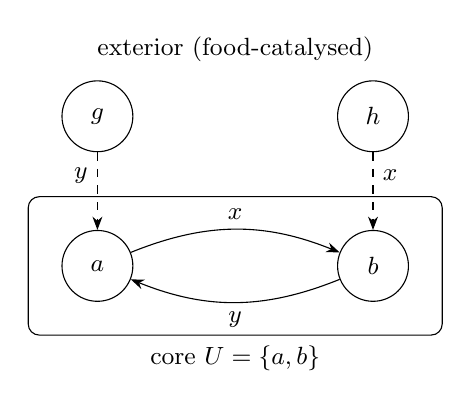
\begin{tikzpicture}[>=Stealth,vertex/.style={circle,draw,minimum size=9mm},every node/.style={font=\small}]
\node[vertex] (a) at (0,0) {$a$};
\node[vertex] (b) at (3.5,0) {$b$};
\node[vertex] (g) at (0,1.9) {$g$};
\node[vertex] (h) at (3.5,1.9) {$h$};
\draw[->] (a) to[bend left=22] node[above] {$x$} (b);
\draw[->] (b) to[bend left=22] node[below] {$y$} (a);
\draw[->,dashed] (g) -- node[pos=.3,left] {$y$} (a);
\draw[->,dashed] (h) -- node[pos=.3,right] {$x$} (b);
\node[draw,rounded corners,fit=(a)(b),inner sep=12pt,label=below:{core $U=\{a,b\}$}] {};
\node at (1.75,2.75) {exterior (food-catalysed)};
\end{tikzpicture}
\caption{Product--catalysis edges in Example~\ref{ex:switch}: an arrow $p\to r$ labelled $x$ means that $p$ produces $x$ and $x$ catalyses $r$. Selecting $g$ makes $a$ automatic in that context; selecting $h$ makes $b$ automatic.}
\label{fig:contexts}
\end{figure}

\subsection{Cycles, feedback vertex sets, and disjoint cores}

\begin{definition}\label{def:support-digraph}
The \emph{food-ready support digraph} $\Gamma(\QQ)$ has vertex set the food-ready reactions,
an arc $p\to r$ whenever $\pi(p)\cap C(r)\neq\varnothing$, and a loop at $r$ whenever
$C(r)\cap F\neq\varnothing$.
\end{definition}

\begin{lemma}\label{lem:cycle-core}
The vertex set of any directed cycle of $\Gamma(\QQ)$ (a loop counts as a cycle of length
one) is an elementary core. Conversely every elementary core contains the vertex set of a
directed cycle of $\Gamma(\QQ)$.
\end{lemma}
\begin{proof}
Let $V$ be the vertex set of a directed cycle. It is nonempty and consists of food-ready
reactions, hence food-generated, and $\cl_V(F)=F\cup\pi(V)$. Each $r\in V$ is either
food-catalysed (a loop) or has a cycle predecessor $p\in V$ with $\pi(p)\cap C(r)\neq\varnothing$;
either way $C(r)\cap\cl_V(F)\neq\varnothing$. Conversely if $U$ is an elementary core then
every $r\in U$ has a catalyst in $F\cup\pi(U)$, so $r$ carries a loop or has an in-neighbour
in $U$; following in-neighbours inside the finite set $U$ produces a directed cycle.
\end{proof}

The first half is the elementary-RAF characterisation of~\cite{steel2019autocatalytic}, where
it is also observed that a shortest cycle is a smallest elementary RAF; we return to this in
Section~\ref{sec:algorithms}.

\begin{corollary}[Cycles meet abundant reactions]\label{cor:cycles}
Every directed cycle of $\Gamma(\QQ)$ contains a globally abundant reaction of $\QQ$.
Hence the subgraph of $\Gamma(\QQ)$ induced by the strictly rare food-ready reactions is
acyclic, the abundant food-ready reactions form a directed feedback vertex set of
$\Gamma(\QQ)$, and if $\Gamma(\QQ)$ has $k$ vertex-disjoint directed cycles then $\QQ$ has at
least $k$ distinct abundant reactions. More generally, pairwise disjoint elementary cores
$U_1,\dots,U_k$ admit distinct abundant reactions $r_i\in U_i$.
\end{corollary}
\begin{proof}
By Lemma~\ref{lem:cycle-core} and Theorem~\ref{thm:core} applied in the full system $\QQ$,
each cycle contains an abundant reaction. A cycle consisting of strictly rare reactions is
therefore impossible, which is the acyclicity and feedback-vertex-set statement. For
disjoint cores choose a witness in each; disjointness makes the choices distinct.
\end{proof}

In particular the number of abundant reactions is at least the minimum size of a directed
feedback vertex set of $\Gamma(\QQ)$. We do not claim that this minimum, or a maximum cycle
packing, is computed by the greedy procedure of Section~\ref{sec:algorithms}.

\subsection{Few non-food-ready reactions}

The following set-family lemma is independent of RAF semantics.

\begin{lemma}[Two-element transversals]\label{lem:transversal}
Let $\FF\subseteq2^R$ be union-closed with $\varnothing\in\FF$ and at least one nonempty member,
$N=|\FF|$. If there are $a,b\in R$ (not necessarily distinct) such that every nonempty member
of $\FF$ contains $a$ or $b$, then $2f(a)\ge N$ or $2f(b)\ge N$.
\end{lemma}
\begin{proof}
Let $\FF_a,\FF_b$ be the members containing $a$, resp.\ $b$; then
$\FF_a\cup\FF_b=\FF\setminus\{\varnothing\}$ has $N-1$ elements. If $\FF_b=\varnothing$ then
$f(a)=N-1\ge N/2$ since $N\ge2$; similarly if $\FF_a=\varnothing$. Otherwise pick
$A\in\FF_a$, $B\in\FF_b$; by union closure $A\cup B\in\FF_a\cap\FF_b$, so
\[
f(a)+f(b)=|\FF_a\cup\FF_b|+|\FF_a\cap\FF_b|\ \ge\ (N-1)+1=N,
\]
and one of $f(a),f(b)$ is at least $N/2$.
\end{proof}

\begin{corollary}[At most two non-food-ready reactions]\label{cor:two}
If a finite CRS has a RAF and at most two of its reactions are not food-ready, then some
reaction is abundant.
\end{corollary}
\begin{proof}
Let $H$ be the set of non-food-ready reactions, $|H|\le2$. If some RAF avoids $H$ it is an
elementary core and Theorem~\ref{thm:core} applies. Otherwise every nonempty member of $\FF$
meets $H$; if $H=\{a,b\}$ (or $H=\{a\}$, taking $b=a$) Lemma~\ref{lem:transversal} applies.
The case $H=\varnothing$ falls under the first branch.
\end{proof}

The overlap term $|\FF_a\cap\FF_b|\ge1$ in Lemma~\ref{lem:transversal} is exactly what pays
for the empty set in the denominator. The same argument does not extend to three exceptional
reactions: a three-element transversal of the nonempty members gives only
$f(a)+f(b)+f(c)\ge N-1+\text{(overlaps)}$, and the average $(N-1)/3$ is well below $N/2$.
We show in Section~\ref{sec:pair} that no argument confined to the non-food-ready
reactions can work in general.

\subsection{Sharpness, intervention, and a feedback example}

\begin{example}[Sharpness]\label{ex:sharp}
Let $U=\{r_1,\dots,r_k\}$ with $r_i:\ f\to c_i$ catalysed only by $c_{i-1}$ (indices modulo
$k$), and no other reactions. Any nonempty RAF containing $r_i$ must contain $r_{i-1}$, hence
all of $U$; so $\FF=\{\varnothing,U\}$, $N=2$ and $f(r_i)=1$ for all $i$. The constant $1/2$
in Theorem~\ref{thm:core} cannot be improved, even for isolated elementary systems.
(This is an existence statement about equality, not a classification of equality cases;
Example~\ref{ex:switch} attains equality with nontrivial exterior support.)
\end{example}

\begin{remark}[Intervention stability]
Theorem~\ref{thm:core} is a statement about one system at a time, so it applies to a
modified system as soon as the core data survive. Deleting exterior reactions, adding
reactions with arbitrary reactants and products, adding catalytic feedback into the core,
enlarging the food set or adding catalysts all preserve the hypotheses on $U$, and each
resulting system has an abundant reaction in $U$. The identity of the witness and the
individual frequencies may change, and no monotonicity of any single $f(r)$ is asserted.
\end{remark}

\begin{example}[Genuine feedback into a viable core]\label{ex:feedback}
Let $F=\{f\}$ and
\[
a:\ f\to c_a\ [c_b],\qquad b:\ f\to \{c_b,z\}\ [c_a],\qquad g:\ z\to\{c_b,d\}\ [f],
\]
brackets giving the catalysts. The core $\{a,b\}$ is an elementary core; $g$ is not
food-ready, consumes the core product $z$, and feeds the catalyst $c_b$ of $a$ back into the
core. The RAF family is $\FF=\{\varnothing,\{a,b\},\{a,b,g\}\}$: $g$ cannot be enabled
without $b$, and $a$ without $b$ has no catalyst other than through $g$. So $N=3$,
$f(a)=f(b)=2$, $f(g)=1$, and $a,b$ are abundant as Theorem~\ref{thm:core} predicts.
This literal example is compiled in the formal development as a consumer of the general
theorem (Appendix~\ref{app:lean}).
\end{example}

\begin{example}[The average over a maximal RAF can fall below one half]\label{ex:false-average}
Let $F=\{f\}$ and $a:\ f\to z\ [f]$, $g:\ z\to c_g\ [c_l]$, $l:\ f\to c_l\ [c_g]$. Then
$\FF=\{\varnothing,\{a\},\{a,g,l\}\}$, $N=3$, and $(f(a),f(g),f(l))=(2,1,1)$. The maximal RAF
$\{a,g,l\}$ has total incidence $4<\tfrac32\cdot3$, so the average frequency over a maximal
RAF, or over all food-ready reactions ($a$ and $l$: average $3/2$, exactly the bound), is not
what the theorem controls. The half-occupancy statement is attached to a viable elementary
core (here $\{a\}$), and the aggregate bound~\eqref{eq:global} concerns incidences in that
core only.
\end{example}

\section{Diagnostics for an embedded module}\label{sec:diagnostics}

Theorem~\ref{thm:core} needs no relation between the isolated behaviour of a module and the
global RAF family. In applications one nevertheless wants to know whether the isolated
analysis of a module is faithful. This section gives an exact, polynomial-time test and a
quantitative version of the abundance bound that separates faithful from unfaithful rows.
Both are formally verified.

Let $E\subseteq R$ be a set of food-ready reactions (a \emph{module}; it need not be a RAF and
may contain reactions that are never active). Define the internal predecessors of $r\in E$ by
\[
P_E(r)=\{p\in E:\ \pi(p)\cap C(r)\neq\varnothing\}.
\]
Say that $E$ is \emph{projection-preserving} if $W\cap E\in\FF$ for every $W\in\FF$.

\begin{theorem}[Exact projection criterion]\label{thm:projection}
$E$ is projection-preserving if and only if for every $r\in E$ with $C(r)\cap F=\varnothing$,
\[
r\notin\mraf_\QQ\bigl(R\setminus P_E(r)\bigr).
\]
If the test fails for $r$, then $W=\mraf_\QQ(R\setminus P_E(r))$ is a RAF containing $r$
whose projection $W\cap E$ is not in $\FF$.
\end{theorem}
\begin{proof}
For any $W\subseteq R$ the set $W\cap E$ is food-generated because its reactions are
food-ready, so by~\eqref{eq:products} $W\cap E\in\FF$ iff every $r\in W\cap E$ has a
catalyst in $F\cup\pi(W\cap E)$, i.e.\ iff $C(r)\cap F\neq\varnothing$ or
$W\cap P_E(r)\neq\varnothing$ for every $r\in W\cap E$.

Suppose the test fails: $r\in E$, $C(r)\cap F=\varnothing$ and $r\in W:=\mraf_\QQ(R\setminus P_E(r))$.
Then $W$ is a RAF with $W\cap P_E(r)=\varnothing$ and $r\in W\cap E$, so $W\cap E\notin\FF$
and $E$ is not projection-preserving; this also proves the witness statement. Conversely
suppose every test passes and let $W\in\FF$, $r\in W\cap E$ with $C(r)\cap F=\varnothing$.
If $W\cap P_E(r)=\varnothing$ then $W$ is a nonempty RAF inside $R\setminus P_E(r)$, so
$r\in W\subseteq\mraf_\QQ(R\setminus P_E(r))$, contradicting the test. Hence
$W\cap P_E(r)\neq\varnothing$ and $W\cap E\in\FF$.
\end{proof}

Each test is one maxRAF computation on a restricted availability set, hence polynomial by
the RAF algorithm~\cite{hordijk2004detecting}. A sufficient condition, requiring no
computation, is that no reaction outside $E$ produces a catalyst of a core reaction that
is not food-catalysed. Example~\ref{ex:feedback} shows that this sufficient condition can
fail while the exact criterion passes: $g\notin E$ produces the catalyst $c_b$ of $a$, but
$\mraf(R\setminus P_E(a))=\mraf(\{a,g\})=\varnothing$ because $g$ needs $z$ from $b$.

\begin{theorem}[Defect bound]\label{thm:defect}
Let $E$ be a module of food-ready reactions with $U=\mraf_\QQ(E)\neq\varnothing$, and let
$\DD_{\rm bad}=\{W\in\FF:\ W\cap E\notin\FF\}$. Then
\begin{equation}\label{eq:defect}
2\sum_{W\in\FF}|W\cap U|\ \ge\ |U|\bigl(N-|\DD_{\rm bad}|\bigr)+2\sum_{W\in\DD_{\rm bad}}|W\cap U| ,
\end{equation}
and consequently some $r\in U$ satisfies
$2|U|\,f(r)\ge|U|(N-|\DD_{\rm bad}|)+2\sum_{W\in\DD_{\rm bad}}|W\cap U|$.
\end{theorem}
\begin{proof}
Let $\GG=\FF\setminus\DD_{\rm bad}$ be the good rows. For $W\in\GG$, $W\cap E$ is empty or a
RAF contained in $E$, hence $W\cap E\subseteq\mraf_\QQ(E)=U$, so $W\cap E=W\cap U$ and
$T:=W\setminus U$ is disjoint from $E$. Fix $T\subseteq R\setminus E$ and consider the good
fibre $\GG_T=\{S\subseteq U:\ S\cup T\in\FF,\ S\in\FF\}$; the map $W\mapsto(W\setminus U,W\cap U)$
is a bijection from $\GG$ onto $\bigsqcup_{T\cap E=\varnothing}\GG_T$.

Since $U$ is an elementary core, define bodies as in the proof of Theorem~\ref{thm:core}
with $T=\varnothing$: $B^0_r=\{r\}$ if $C(r)\cap F\neq\varnothing$ and
$B^0_r=\{p\in U:\pi(p)\cap C(r)\neq\varnothing\}$ otherwise; these are nonempty. For
$S\subseteq U$, $S\in\FF$ iff $S\cap B^0_r\neq\varnothing$ for all $r\in S$. Given $S\in\FF$,
the condition $S\cup T\in\FF$ reduces to $K_T(S)$ of Theorem~\ref{thm:core}, because the
support of the reactions of $S$ inside $F\cup\pi(S)$ persists in $F\cup\pi(S\cup T)$. Hence
$\GG_T=\{S\subseteq U: K_T(S),\ S\cap B^0_r\neq\varnothing\ \forall r\in S\}$ and
Lemma~\ref{lem:count} gives $\sum_{S\in\GG_T}(2|S|-|U|)\ge0$. Summing over $T$,
$2\sum_{W\in\GG}|W\cap U|\ge|U|\,|\GG|=|U|(N-|\DD_{\rm bad}|)$. Adding the bad rows
gives~\eqref{eq:defect}, and $\sum_W|W\cap U|=\sum_{r\in U}f(r)\le|U|\max_{r\in U}f(r)$ gives
the frequency form.
\end{proof}

The bound~\eqref{eq:defect} reproduces~\eqref{eq:global} when $\DD_{\rm bad}=\varnothing$ and
is weaker than it in general (it discards the good half-occupancy in bad rows in exchange
for their exact incidence). Its use is descriptive: it tells how much of the core incidence
is contributed by rows in which the module's isolated analysis is unfaithful.

\begin{example}[Projection fails, abundance holds, the defect bound is tight]\label{ex:failed-projection}
Let $F=\{f\}$ and $a:\ f\to u\ [f]$, $b:\ f\to z\ [c]$, $g:\ z\to c\ [f]$, with module
$E=\{a,b\}$. Isolated, $U=\mraf(E)=\{a\}$, because $c$ is not produced inside $E$. Globally
$\FF=\{\varnothing,\{a\},\{b,g\},\{a,b,g\}\}$: the pair $\{b,g\}$ is a RAF in which $g$
consumes $z$ from $b$ and returns the catalyst $c$. Projection fails,
$\{b,g\}\cap E=\{b\}\notin\FF$, and the deletion query for $b$ (with $P_E(b)=\varnothing$)
returns the witness $\mraf(R)=\{a,b,g\}$. Here $N=4$, $f(a)=f(b)=f(g)=2$,
$\DD_{\rm bad}=\{\{b,g\},\{a,b,g\}\}$, and~\eqref{eq:defect} reads $4\ge1\cdot2+2\cdot1=4$.
\end{example}

\begin{remark}[Layer identities]
For a distinguished reaction $g$, the rows omitting $g$ and the rows containing $g$ with
$g$ erased partition the incidence counts exactly: $N=|\FF_{\bar g}|+|\FF_g|$, $f(g)=|\FF_g|$,
and $f(r)=f_{\bar g}(r)+f_g(r)$ for $r\neq g$, where erasure is injective on rows containing
$g$. These identities are useful when testing proposed extension inequalities and are part
of the formal development, but the proof of Theorem~\ref{thm:core} does not need them.
\end{remark}

\section{Realisation of RAF interior operators on a fixed reaction set}\label{sec:realization}

We now ask which interior operators arise as $\mraf_\QQ$. The answer separates the two
halves of RAF semantics: food generation, which is an antimatroid, and catalytic support,
which is a predecessor condition.

\subsection{Blockers}

Let $\DD\subseteq2^V$ be union-closed with $\varnothing\in\DD$ and interior $i_\DD$.

\begin{definition}
For $v\in V$, a \emph{blocker} for $v$ is a set $B\subseteq V$ with $v\notin B$ and
$v\notin i_\DD(V\setminus B)$. Write $\HH_v$ for the set of blockers of $v$. The empty set is
a blocker for $v$ exactly when $v$ lies in no member of $\DD$.
\end{definition}

\begin{lemma}[Blocker test]\label{lem:block}
For $v\in A\subseteq V$: $v\in i_\DD(A)$ if and only if $A\cap B\neq\varnothing$ for every
$B\in\HH_v$.
\end{lemma}
\begin{proof}
If $A\cap B=\varnothing$ for a blocker $B$ then $A\subseteq V\setminus B$ and monotonicity gives
$i_\DD(A)\subseteq i_\DD(V\setminus B)\not\ni v$. Conversely if $v\notin i_\DD(A)$ then
$V\setminus A$ is a blocker for $v$ disjoint from $A$.
\end{proof}

\begin{lemma}[Minimal blockers suffice]\label{lem:minimal}
Every blocker for $v$ contains an inclusion-minimal blocker for $v$, so the test of
Lemma~\ref{lem:block} may be restricted to minimal blockers. Every blocker is contained in
$V\setminus\{v\}$, so $|\HH_v|\le2^{|V|-1}$ and $\sum_{B\in\HH_v}|B|\le(|V|-1)|\HH_v|$.
\end{lemma}
\begin{proof}
Among the blockers contained in a given blocker choose one of minimum cardinality. The
bounds are immediate.
\end{proof}

Minimality does not make the blocker description polynomial. For the threshold family
$\DD=\{\varnothing\}\cup\{A\subseteq V:|A|\ge k\}$ on $n$ elements, $B$ is a blocker for $v$ iff
$v\notin B$ and $|V\setminus B|<k$, so the minimal blockers for $v$ are exactly the
$(n-k+1)$-subsets of $V\setminus\{v\}$, of which there are $\binom{n-1}{n-k+1}$.

\subsection{Exact-ground characterisation}

Call $\AAf\subseteq2^V$ an \emph{antimatroid family} if $\varnothing\in\AAf$, $\AAf$ is
union-closed, and $\AAf$ is \emph{accessible}: every nonempty $S\in\AAf$ has an element $v$
with $S\setminus\{v\}\in\AAf$. We do not require $\bigcup\AAf=V$, so elements that lie in no
member are allowed; up to this convention these are the feasible-set families of
antimatroids~\cite{dilworth1940lattices,korte1991greedoids}.

\begin{lemma}[Food generation is accessible]\label{lem:accessible}
For any finite CRS, the family of food-generated subsets of $R$ is an antimatroid family.
\end{lemma}
\begin{proof}
It contains $\varnothing$ and is union-closed by monotonicity of closure. Let $S$ be
nonempty and food-generated, and for $r\in S$ let $j(r)$ be the least $j$ with
$\rho(r)\subseteq L_j(S)$. Choose $v\in S$ with $j(v)$ maximal. By induction on $j\le j(v)$
one has $L_j(S\setminus\{v\})=L_j(S)$: the recursion for $L_{j+1}$ with $j<j(v)$ only uses
reactions enabled at $L_j(S)$, and $v$ is not among them. Hence every $r\in S\setminus\{v\}$
has $\rho(r)\subseteq L_{j(r)}(S)=L_{j(r)}(S\setminus\{v\})$, and $S\setminus\{v\}$ is
food-generated.
\end{proof}

\begin{theorem}[Exact-ground realisability]\label{thm:same}
An interior operator $\psi$ on $2^V$, $V$ finite, is the RAF interior operator
$\mraf_\QQ$ of a finite CRS $\QQ$ with reaction set exactly $V$ if and only if there exist
an antimatroid family $\AAf\subseteq2^V$ and a map $P:V\to2^V$ such that
\begin{equation}\label{eq:same}
\Fix(\psi)=\{S\in\AAf:\ S\cap P(v)\neq\varnothing\ \text{for every } v\in S\}.
\end{equation}
\end{theorem}
\begin{proof}
\emph{Necessity.} Let $\AAf$ be the food-generated subsets of $R=V$, an antimatroid family by
Lemma~\ref{lem:accessible}, and let $P(v)=\{p\in V:\pi(p)\cap C(v)\neq\varnothing\}$, with $v$
adjoined to $P(v)$ when $C(v)\cap F\neq\varnothing$. By~\eqref{eq:products}, a food-generated
$S$ is empty or a RAF iff every $v\in S$ has a catalyst in $F\cup\pi(S)$, iff
$S\cap P(v)\neq\varnothing$ for every $v\in S$. This is~\eqref{eq:same} with $\Fix(\psi)=\FF(\QQ)$.

\emph{Sufficiency.} Given $\AAf$ and $P$, let $\HH_v$ be the blockers of $v$ with respect
to $\AAf$. Take molecules: one food molecule $f$, a private product $c_v$ for each $v\in V$,
and a marker $m_{v,B}$ for each $v\in V$ and $B\in\HH_v$. Define, for each $v\in V$, the
single reaction
\begin{equation}\label{eq:marker}
v:\quad \{f\}\cup\{m_{v,B}:B\in\HH_v\}\ \longrightarrow\ \{c_v\}\cup\{m_{u,B}:\ u\in V,\ B\in\HH_u,\ v\in B\},
\end{equation}
catalysed exactly by the molecules $c_p$, $p\in P(v)$. Thus the marker $m_{u,B}$ is produced
precisely by the reactions indexed by elements of $B$, and $c_p$ is produced only by $p$.

We show that the food-generated subsets of this system are exactly $\AAf$. Let $S\in\AAf$;
we induct on $|S|$, the case $S=\varnothing$ being trivial. Choose $v\in S$ with
$S\setminus\{v\}\in\AAf$; by induction it is food-generated, so
$\cl_{S\setminus\{v\}}(F)=F\cup\pi(S\setminus\{v\})$. Every reaction of $S\setminus\{v\}$ has
its reactants in $\cl_{S\setminus\{v\}}(F)\subseteq\cl_S(F)$. For $v$: $f\in F$, and for
$B\in\HH_v$ we have $v\in S=i_\AAf(S)$, so $S\cap B\neq\varnothing$ by Lemma~\ref{lem:block};
as $v\notin B$ some $u\in S\setminus\{v\}$ lies in $B$ and produces $m_{v,B}$, so
$m_{v,B}\in\pi(S\setminus\{v\})\subseteq\cl_S(F)$. Hence $S$ is food-generated.

Conversely let $S$ be food-generated and nonempty; we induct on $|S|$. By
Lemma~\ref{lem:accessible} there is $v\in S$ with $S\setminus\{v\}$ food-generated, hence in
$\AAf$ by induction. For $B\in\HH_v$ the marker $m_{v,B}\in\rho(v)\subseteq\cl_S(F)=F\cup\pi(S)$
is not food, so it is produced by some $u\in S$ with $u\in B$; thus $S\cap B\neq\varnothing$
for all $B\in\HH_v$, and Lemma~\ref{lem:block} gives $v\in i_\AAf(S)$. Also
$S\setminus\{v\}\in\AAf$ and $S\setminus\{v\}\subseteq S$ give $S\setminus\{v\}\subseteq i_\AAf(S)$.
So $i_\AAf(S)=S$ and $S\in\AAf$. (This direction is what excludes circular marker
bootstrapping: a set of reactions that merely produce one another's markers is not
food-generated unless some admissible order exists.)

Finally, for a food-generated $S$ the molecule $c_p$ lies in $\cl_S(F)=F\cup\pi(S)$ iff
$p\in S$, so $S$ is empty or a RAF iff $S\in\AAf$ and $S\cap P(v)\neq\varnothing$ for every
$v\in S$. The fixed family of $\mraf_\QQ$ is therefore the right-hand side
of~\eqref{eq:same}, which equals $\Fix(\psi)$, and interior operators with equal fixed
families are equal.
\end{proof}

\begin{corollary}[Food generation is exactly antimatroidal]\label{cor:antimatroid}
A family $\AAf\subseteq2^V$ is the family of food-generated subsets of some finite CRS with
reaction set $V$ if and only if $\AAf$ is an antimatroid family.
\end{corollary}
\begin{proof}
Lemma~\ref{lem:accessible} and the first part of the sufficiency proof of
Theorem~\ref{thm:same}, which did not use catalysis.
\end{proof}

Theorem~\ref{thm:same} is a structural factorisation of RAF realisability, not an efficient
algorithm for finding a factorisation of a family given explicitly; the marker construction
may have exponentially many markers (Lemma~\ref{lem:minimal} and the threshold example).
It uses $1+|V|+b$ molecules and $2|V|+b+j+\sum_v|P(v)|$ reactant, product and catalyst
incidences, where $b=\sum_v|\HH_v|$ and $j=\sum_v\sum_{B\in\HH_v}|B|$.

\section{Sparse universality and the union-closed boundary}\label{sec:pair}

Theorem~\ref{thm:same} shows that not every interior operator is a RAF interior operator on
the same ground set: the fixed family must be an antimatroid family cut down by predecessor
support, and a union-closed family with no accessible structure (for instance
$\{\varnothing\}\cup\{A:|A|\ge2\}$) is not of this form. Allowing two reactions per coordinate
removes the restriction entirely, and does so with a very sparse catalytic structure.

\begin{construction}[Producer--gate source]\label{con:pair}
Let $\DD\subseteq2^V$ be union-closed with $\varnothing\in\DD$, with blockers $\HH_v$ as in
Section~\ref{sec:realization}. Take one food molecule $f$, private molecules
$\alpha_v,\beta_v$ for $v\in V$, and markers $m_{v,B}$ for $B\in\HH_v$. For each $v$ take two
reactions,
\begin{align}
p_v:&\quad f\ \longrightarrow\ \{\alpha_v\}\cup\{m_{u,B}:\ B\in\HH_u,\ v\in B\} &&\text{catalysed only by }\beta_v,\label{eq:producer}\\
g_v:&\quad \{f\}\cup\{m_{v,B}:B\in\HH_v\}\ \longrightarrow\ \{\beta_v\} &&\text{catalysed only by }\alpha_v.\label{eq:gate}
\end{align}
Call the resulting CRS $\QQ_\DD$. For $A\subseteq V$ put $\enc(A)=\{p_v,g_v:v\in A\}$, and for
a set $T$ of reactions of $\QQ_\DD$ let $c(T)=\{v:\ p_v\in T\text{ and }g_v\in T\}$ be its
\emph{complete pairs}.
\end{construction}

\begin{figure}[tb]\centering
\begin{tikzpicture}[>=Stealth,every node/.style={font=\small},rx/.style={draw,rectangle,minimum width=10mm,minimum height=8mm}]
\node[rx] (p) at (0,0) {$p_v$};
\node[rx] (g) at (5.2,0) {$g_v$};
\node (f1) at (-1.7,0) {$f$};
\node (m) at (5.2,1.4) {$f,\ \{m_{v,B}\}_{B\in\HH_v}$};
\node (alpha) at (1.9,.95) {$\alpha_v$};
\node (beta) at (3.3,-.95) {$\beta_v$};
\node (marks) at (0,-1.5) {$\{m_{u,B}: v\in B\}$};
\draw[->] (f1)--(p);
\draw[->] (p)--(alpha);
\draw[->,dashed] (alpha)--(g);
\draw[->] (g)--(beta);
\draw[->,dashed] (beta)--(p);
\draw[->] (m)--(g);
\draw[->] (p)--(marks);
\end{tikzpicture}
\caption{One producer--gate pair of Construction~\ref{con:pair}. Solid arrows are reactant and product relations, dashed arrows catalysis. The producer is food-ready and emits its marker outputs in the first closure round; the gate is enabled exactly when every blocker of $v$ meets the selected coordinates.}
\label{fig:pair}
\end{figure}

\begin{theorem}[Sparse two-round universality]\label{thm:pair}
For every finite union-closed $\DD\subseteq2^V$ containing $\varnothing$:
\begin{enumerate}[label=(\roman*)]
\item $\FF(\QQ_\DD)=\{\enc(A):A\in\DD\}$, and $\enc$ is a bijection from $\DD$ onto
$\FF(\QQ_\DD)$ that preserves inclusions and unions; in particular
$f(p_v)=f(g_v)=|\{A\in\DD:v\in A\}|$ for every $v$.
\item For every set $T$ of reactions of $\QQ_\DD$, $\mraf_{\QQ_\DD}(T)=\enc\bigl(i_\DD(c(T))\bigr)$.
\item $\QQ_\DD$ has $2|V|$ reactions, one food molecule, exactly one catalyst per reaction,
no self-catalysis, and its product--catalysis arcs are exactly the two-cycles
$p_v\leftrightarrow g_v$.
\item For every set $T$ of reactions, $L_{j+2}(T)=L_2(T)$ for all $j\ge0$.
\end{enumerate}
\end{theorem}
\begin{proof}
(i) The only source of $\beta_v$ is $g_v$ and the only source of $\alpha_v$ is $p_v$;
neither is food. In a RAF $W$, $p_v\in W$ needs $\beta_v$ in the closure, hence $g_v\in W$,
and $g_v\in W$ needs $\alpha_v$, hence $p_v\in W$. So every RAF is $\enc(A)$ for a unique
nonempty $A$. Now fix $A\subseteq V$ nonempty and consider $\enc(A)$. All producers are
food-ready, so $L_1(\enc(A))$ contains $f$, all $\alpha_v$ ($v\in A$), and exactly the
markers $m_{u,B}$ with $B\cap A\neq\varnothing$. Markers have no other source, so $g_v$
($v\in A$) is ever enabled iff $A\cap B\neq\varnothing$ for all $B\in\HH_v$, iff
$v\in i_\DD(A)$ by Lemma~\ref{lem:block}. Hence $\enc(A)$ is food-generated iff
$A\subseteq i_\DD(A)$, iff $A\in\DD$. When $A\in\DD$, all $\beta_v$ ($v\in A$) appear in
$L_2$, and every reaction of $\enc(A)$ has its catalyst in the closure, so $\enc(A)$ is a
RAF; when $A\notin\DD$ it is not even food-generated. Together with
$\enc(\varnothing)=\varnothing\in\FF$ this proves (i); frequency preservation follows from
the bijection, since $p_v,g_v\in\enc(A)$ iff $v\in A$.

(ii) The RAFs contained in $T$ are the sets $\enc(A)$ with $A\in\DD$ and $\enc(A)\subseteq T$,
i.e.\ $A\subseteq c(T)$. Their union is $\enc$ of the union of the members of $\DD$ inside
$c(T)$, which is $\enc(i_\DD(c(T)))$ because $\enc$ commutes with unions. A producer whose
gate is unavailable (or vice versa) contributes nothing, as it must: an incomplete pair
never lies in a RAF.

(iii) is read off from~\eqref{eq:producer}--\eqref{eq:gate}: the only product of $g_v$ is
$\beta_v$, which catalyses only $p_v$; among the products of $p_v$ only $\alpha_v$ is a
catalyst, and it catalyses only $g_v$; markers catalyse nothing.

(iv) Let $T$ be any set of reactions. Every producer in $T$ is enabled at stage $0$, so
$L_1(T)$ contains all markers and all $\alpha$'s that will ever be produced. A gate's
reactants are $f$ and markers, so every gate in $T$ that is ever enabled is enabled at
$L_1(T)$ and its output $\beta$ lies in $L_2(T)$. Gate outputs are never reactants. Hence
$L_3(T)=L_2(T)$, and by induction $L_{j+2}(T)=L_2(T)$. Nothing here requires $T$ to be
paired or a RAF.
\end{proof}

\begin{proposition}[Elementary RAFs of the universal source]\label{prop:paircore}
Let $E_{\rm food}$ be the set of food-ready reactions of $\QQ_\DD$ and
$J=\{v\in V:\{v\}\in\DD\}$. A gate $g_v$ is food-ready iff $\{v\}\in\DD$, and
\begin{equation}\label{eq:paircore}
\mraf_{\QQ_\DD}(E_{\rm food})=\enc(J).
\end{equation}
In particular $\QQ_\DD$ has an elementary RAF if and only if $\DD$ has a singleton member,
and its elementary RAFs are exactly the encodings of the members of $\DD$ contained in $J$.
\end{proposition}
\begin{proof}
Producers are always food-ready; $g_v$ is food-ready iff it has no marker reactants, iff
$\HH_v=\varnothing$. If $\{v\}\in\DD$ then for every $B\not\ni v$ the member $\{v\}\subseteq V\setminus B$
witnesses $v\in i_\DD(V\setminus B)$, so $\HH_v=\varnothing$. If $\HH_v=\varnothing$ then
Lemma~\ref{lem:block} at $A=\{v\}$ gives $v\in i_\DD(\{v\})$, so $\{v\}\in\DD$. Thus
$c(E_{\rm food})=J$. Union closure gives $J\in\DD$ (including $J=\varnothing$), so
Theorem~\ref{thm:pair}(ii) yields~\eqref{eq:paircore}. An elementary RAF is a RAF inside
$E_{\rm food}$, i.e.\ $\enc(A)$ with $A\in\DD$, $A\neq\varnothing$, $A\subseteq J$.
\end{proof}

\subsection{The boundary}

If $\{v\}\in\DD$ then $v$ is abundant in $\DD$: the map $A\mapsto A\cup\{v\}$ injects the
members omitting $v$ into the members containing $v$~\cite{sarvate1989union}. On the
universal source $\QQ_\DD$, therefore, Theorem~\ref{thm:core} says exactly this and nothing
more: an elementary core exists iff a singleton member exists, and then the core is
$\enc(J)$, one of whose coordinates is abundant. The interest of Theorem~\ref{thm:core} lies
in systems that are not of the form $\QQ_\DD$, where elementary cores are common and
carry no singleton information about the family.

Conversely, the class of CRSs \emph{without} an elementary core is as hard as the general
problem.

\begin{theorem}[Equivalence with the union-closed conjecture]\label{thm:equiv}
The following are equivalent.
\begin{enumerate}[label=(\alph*)]
\item Every finite union-closed family $\DD$ with $\varnothing\in\DD$ and a nonempty member has
an element $v$ with $2|\{A\in\DD:v\in A\}|\ge|\DD|$ (Frankl's conjecture).
\item Every finite CRS possessing a RAF has an abundant reaction.
\item Every finite CRS possessing a RAF, with one food molecule, one catalyst per reaction, no
self-catalysis, product--catalysis arcs forming disjoint two-cycles, two-round closure
stabilisation, and no elementary RAF, has an abundant reaction.
\end{enumerate}
\end{theorem}
\begin{proof}
(a)$\Rightarrow$(b): $\FF(\QQ)$ is union-closed with $\varnothing\in\FF(\QQ)$ (Lemma~\ref{lem:uc}).
(b)$\Rightarrow$(c) is trivial. (c)$\Rightarrow$(a): let $\DD$ be as in (a). If $\DD$ has a
singleton member, that element is abundant by the injection above. Otherwise $\QQ_\DD$ has
all the properties listed in (c) by Theorem~\ref{thm:pair}(iii),(iv) and
Proposition~\ref{prop:paircore}, and it has a RAF because $\DD$ has a nonempty member.
By (c) some reaction $p_v$ or $g_v$ is abundant in $\FF(\QQ_\DD)$, and by
Theorem~\ref{thm:pair}(i) $|\FF(\QQ_\DD)|=|\DD|$ and $f(p_v)=f(g_v)=|\{A\in\DD:v\in A\}|$, so
$v$ is abundant in $\DD$.
\end{proof}

Theorem~\ref{thm:equiv} constrains further work. Unique catalysts, absence of
self-catalysis, a catalytic graph consisting of private two-cycles, and shallow molecular
closure do not, separately or together, remove the difficulty of the unrestricted
conjecture: the universal source has all of them and carries the whole difficulty in its
reactant requirements. Any additional hypothesis proposed to yield abundance for coreless
systems should first be tested against Construction~\ref{con:pair}; if the universal source
satisfies it, a theorem under that hypothesis is a theorem about all union-closed families.
The two-round stabilisation in Theorem~\ref{thm:pair}(iv) also shows that closure depth
places no bound on the number of non-food-ready reactions, so Corollary~\ref{cor:two} does
not indicate a sharp threshold at three exceptional reactions.

\begin{remark}[Size of the encoding]
$\QQ_\DD$ has a linear number of reactions but $1+2|V|+b$ molecule labels and $6|V|+b+j$
reactant, product and catalyst incidences, where $b=\sum_v|\HH_v|$ and
$j=\sum_v\sum_{B\in\HH_v}|B|$; both can be exponential in $|V|$, and by
Lemma~\ref{lem:minimal} restricting to minimal blockers does not change this in the worst
case. Linear reaction count must not be mistaken for a polynomial-size description. The
formal statement (Appendix~\ref{app:lean}) uses the all-blocker construction; the
minimal-blocker membership test is formalised separately as an equivalence of predicates.
\end{remark}

\section{Certificates and algorithms}\label{sec:algorithms}

The results above suggest a small toolkit for a given finite CRS.

\paragraph{Elementary-core certificates.} Build $\Gamma(\QQ)$ (Definition~\ref{def:support-digraph}).
A shortest directed cycle can be found by breadth-first search from each vertex in time
$O(|V_\Gamma|(|V_\Gamma|+|E_\Gamma|))$. By Lemma~\ref{lem:cycle-core} its vertex set is an
elementary RAF, and it is a smallest elementary RAF by reaction count, since every
elementary RAF contains a cycle~\cite{steel2019autocatalytic}. By Theorem~\ref{thm:core} it
contains a reaction abundant in the whole system. This is a compact certificate: a small set
guaranteed to contain an abundant reaction, produced without enumerating any RAF family.
The certificate does not identify which member is abundant unless it is a singleton (a
food-catalysed or self-catalysed food-ready reaction).

\paragraph{Cycle packing.} Repeatedly extract a shortest cycle and delete its vertices.
The cycles found are vertex-disjoint, so by Corollary~\ref{cor:cycles} their number is a
lower bound on the number of abundant reactions. The greedy packing need not be maximum.

\paragraph{Module diagnostics.} For a module $E$ of food-ready reactions, compute
$U=\mraf_\QQ(E)$ by the RAF algorithm restricted to $E$; if nonempty, $U$ contains an
abundant reaction of the full system (Theorem~\ref{thm:core}, with the isolated maxRAF as
core). Run the $|E|$ deletion queries of Theorem~\ref{thm:projection} to decide whether the
module's isolated analysis is faithful globally, and, if not, obtain an explicit RAF
witnessing the failure. All of this is polynomial in the size of the system.

\paragraph{Benchmarks with known answers.} Construction~\ref{con:pair} turns any explicit
union-closed family into a CRS whose RAF family, frequencies and maxRAF operator are known
exactly, which is useful for validating RAF software; the marker construction of
Theorem~\ref{thm:same} does the same for exact-ground realisations.

\section{Scope and open problems}\label{sec:scope}

The results are statements about finite set families. They assert nothing about
concentrations, fluxes, persistence under dynamics, thermodynamic feasibility, or the
chemical realisability of marker molecules, and a reaction that lies in half of all RAFs is
not thereby essential to any of them. The weighted theorem allows arbitrary nonnegative
weights on exterior contexts but not arbitrary weights on individual RAFs.

The proved sufficient condition for abundance is the existence of a viable elementary core,
supplemented by the one- and two-exception cases, which also cover some coreless systems.
Theorem~\ref{thm:equiv} shows that no condition satisfied by the universal source can be
sufficient short of the full conjecture. Between these lies a range of natural questions.

\begin{question}
Which structural hypotheses on a CRS without an elementary core, not satisfied by
Construction~\ref{con:pair}, imply abundance? Candidates should constrain reactant
requirements, since the construction shows that catalytic structure alone can be made
trivial.
\end{question}

\begin{question}
Classify the systems in which every exterior fibre has zero slack (Remark~\ref{rem:slack}),
and find conditions forcing strictly positive slack, i.e.\ a frequency strictly above $N/2$
in the core.
\end{question}

\begin{question}
When can the witness be narrowed inside the core, or shown to be stable across a specified
family of exterior contexts? Example~\ref{ex:switch} shows that some hypothesis beyond
viability is needed.
\end{question}

\begin{question}
Characterise the union-closed families that admit a producer--gate, or exact-ground,
realisation with polynomially many markers.
\end{question}

The strongest positive statement we know of for general RAF families is the general
constant of the entropy method~\cite{gilmer2022constant,alweiss2022improved,chase2022approximate,sawin2022improved,cambie2022better},
which gives a reaction in a $0.38$ fraction of all RAFs of any CRS with a RAF. Whether the
RAF structure can push that constant to $1/2$ is, by Theorem~\ref{thm:equiv}, exactly the
union-closed sets conjecture.

\appendix

\section{Formal verification}\label{app:lean}

\subsection{Environment and provenance}

The formal development is written in Lean~4 (toolchain \lean{leanprover/lean4:v4.30.0})
against Mathlib at commit \lean{c5ea0035} (the \lean{v4.30.0} tag). Each result below was
compiled with \lean{-DwarningAsError=true}; the compiler produced no output. A verification
receipt records, for each root module, the SHA-256 of the root source, of every local
dependency source and of the Lake manifest, together with an elaboration probe of each
exported declaration. Every exported theorem depends only on the axioms
\lean{Classical.choice}, \lean{Quot.sound} and \lean{propext}; there are no \lean{sorry}s and
no \lean{native_decide}. The receipts used here are:

\begin{center}\small
\begin{tabular}{@{}lll@{}}\toprule
Root module & Exported declarations & Root SHA-256 (prefix)\\\midrule
\lean{RAF/Frankl/StructuralMain.lean} & 11 & \lean{d23caca1b9b9705c}\\
\lean{RAF/Frankl/CoreConsequences.lean} & 3 & \lean{53f5cd106e1e85a5}\\
\lean{RAF/Frankl/PairCore.lean} & 2 & \lean{c6e1118ff58e6fc}\\
\lean{RAFInteriorRealizability/Corollaries.lean} & 3 & \lean{96128a929c660aa4}\\\bottomrule
\end{tabular}
\end{center}

The RAF semantics is defined literally as in Definition~\ref{def:crs}: a structure
\texttt{CRS M R} with \lean{food}, \lean{inputs} and \lean{outputs}, a relation
\texttt{Catalysis M R}, the iterated closure \texttt{closureAt Q S k}, the predicates
\lean{FoodGenerated}, \lean{CatalyzedFromClosure} and \lean{IsRAF}, the finite families
\lean{rafFamily} and \lean{fixedFamily} (the latter is $\FF$), and \lean{frequency}. A
food-ready reaction is a \lean{SeedReaction}. The executable maxRAF used in the
projection results is \lean{RAFQueryCompilation.evaluate}, the iterated pruning operator of
the RAF algorithm, proved to compute the largest RAF inside its argument.

\subsection{Correspondence}

\begin{center}\small
\renewcommand{\arraystretch}{1.12}
\begin{tabular}{@{}>{\raggedright\arraybackslash}p{.36\linewidth}>{\raggedright\arraybackslash}p{.58\linewidth}@{}}\toprule
Article statement & Lean declaration (namespace \lean{RAF.Frankl} unless stated)\\\midrule
Lemma~\ref{lem:count} & \lean{supported_upward_average} (module \lean{ElementaryConditioning}); the injection is \lean{conditionedCellMap} with \lean{conditionedCellMap_injOn}\\
Theorem~\ref{thm:core}, identity~\eqref{eq:exact-fibre} & \lean{extension_fibre_iff}\\
Theorem~\ref{thm:core}, fibre inequality~\eqref{eq:fibre} & \lean{extensionFibre_average}\\
Theorem~\ref{thm:core}, global witness & \lean{elementary_core_exists_abundant}; fibre summation is \lean{exists_frequency_of_fibre_average}\\
Theorem~\ref{thm:core}, empty-inclusive form & \lean{elementary_core_rafFixedFrankl}\\
Corollary~\ref{cor:weight}, inequality~\eqref{eq:weight} & \lean{exterior_weighted_fibre_average} (real weights, fibre-indexed)\\
Corollary~\ref{cor:cycles}, cycle vertex sets & \lean{supported_food_ready_abundant} (support predicate \lean{ProductGraphCatalyzed})\\
Corollary~\ref{cor:cycles}, disjoint cores & \lean{disjoint_elementary_cores_distinct_abundant}\\
Lemma~\ref{lem:transversal} (RAF form) & \lean{two_hit_rafFixedFrankl}\\
Corollary~\ref{cor:two} & \lean{one_nonfood_rafFixedFrankl}, \lean{two_nonfood_rafFixedFrankl}\\
Example~\ref{ex:feedback} & \lean{ExtensionExample.abundant_core_reaction}\\
Theorem~\ref{thm:projection} & \lean{projection_iff_deletion_queries}, \lean{failed_query_witness}\\
Isolated maxRAF as core & \lean{elementary_maxRAF_exists_abundant}\\
Theorem~\ref{thm:defect} & \lean{feedback_defect_bound}, \lean{feedback_defect_frequency}\\
Layer identities & \lean{layer_card_identity}, \lean{layer_frequency_identity}\\
Lemma~\ref{lem:block} & \lean{UnionClosedData.mem_interior_iff_hits_blockers}\\
Lemma~\ref{lem:minimal} & \lean{UnionClosedData.mem_interior_iff_hits_minimal_blockers}, \lean{blocker_card_bound}, \lean{marker_output_incidence_bound}\\
Lemma~\ref{lem:accessible} & \lean{RAF.foodGenerated_accessible}\\
Theorem~\ref{thm:same} & \lean{RAFInteriorRealizability.rafInteriorOperator_realizable_iff}\\
Corollary~\ref{cor:antimatroid} & \lean{RAFInteriorRealizability.foodGenerationFamilyRealizable_iff_antimatroid}\\
Theorem~\ref{thm:pair} & \lean{PairGadget.sparse_two_round_realization}\\
Proposition~\ref{prop:paircore} & \lean{PairGadget.gate_food_ready_iff_singleton}, \lean{PairGadget.evaluate_food_ready_eq_singletons}\\
Theorem~\ref{thm:equiv}, (a)$\Leftrightarrow$(b) & \lean{PairGadget.all_rafFixedFrankl_iff_all_unionClosedFrankl}\\
Molecule count of $\QQ_\DD$ & \lean{PairGadget.declared_molecule_count}\\\bottomrule
\end{tabular}
\end{center}

\subsection{What is and is not formalised}

The formal statements are literal. In particular, \lean{elementary_core_exists_abundant}
takes an arbitrary \lean{CRS}, an arbitrary catalysis relation, a finite set \lean{U} with
\texttt{IsRAF Q C U} and every element a \lean{SeedReaction}, and returns
$r\in U$ with $|\FF|\le2f(r)$ for the full system; no projection or feedback hypothesis
appears. The weighted export is the weighted sum of fibre inequalities over an explicit
finite set of contexts; the reindexing by $W\mapsto W\setminus U$ and the weighted witness
deduction in Corollary~\ref{cor:weight} are ordinary mathematics in this paper. The cycle
corollary is connected through the food/product support predicate on a vertex set rather
than through a graph-library notion of cycle; Lemma~\ref{lem:cycle-core} is proved here.
The formal version of Lemma~\ref{lem:transversal} is stated for RAF families.
Theorem~\ref{thm:equiv}(c) is a paper corollary of the formal (a)$\Leftrightarrow$(b) and the
formal properties of the universal source. Examples~\ref{ex:switch}, \ref{ex:sharp},
\ref{ex:false-average} and~\ref{ex:failed-projection}, the threshold-family blocker count,
the incidence formulas, and the feedback-vertex-set remark are checked by hand (the
examples also by exhaustive enumeration in an independent script); Example~\ref{ex:feedback}
is compiled. The shortest-cycle and packing procedures of Section~\ref{sec:algorithms} are
ordinary algorithms whose correctness follows from the theorems; the accompanying
implementation is validated by tests against exhaustive enumeration on small systems, not by
kernel certificates.

\section*{Acknowledgements}
To be inserted.

\bibliographystyle{plainnat}
\bibliography{refs}

\end{document}
